\part{血液系统疾病急诊}

\chapter{急性出血性疾病}

\section{原发性血小板减少性紫癜}

原发性血小板减少性紫癜(primary idiopathic thrombocytopenic
purpura,PITP),或称特发性血小板减少性紫癜(idiopathic thrombocytopenic
purpura,ITP),是一种原因不明的单独血小板减少的一类获得性疾病。属自身免疫性疾病。存在于患者血清中的血小板抗体,使血小板在单核-巨噬细胞系统(主要是脾脏)容易被破坏。在临床主要表现为广泛皮肤黏膜出血、血小板减少、骨髓巨核细胞发育成熟障碍、血小板生存时间缩短及血小板膜糖蛋白特异性自身抗体出现等。ITP的发病率为5~10/10万人口,是常见的出血性疾病之一。临床上分急性与慢性两型。前者好发于儿童,后者多见于成人。男女发病率相近,育龄期女性发病率高于同年龄段男性。

\subsection{病因与发病机制}

ITP的病因未明。目前认为相关发病机制包括:

\paragraph{感染}

急性型多发生于病毒感染恢复期,可能是:①病毒抗原与相关抗体形成免疫复合物附着于血小板表面,促进血小板破坏。②病毒组分结合于血小板表面后,使其抗原性发生改变,导致自身抗体形成,使血小板受损,故可能为感染后的自身免疫反应。

\paragraph{免疫因素}

慢性型60\%~85\%患者的血清中可测出抗血小板抗体;这类抗体多属IgG,损伤血小板,使其寿命缩短,并证明抗体为针对血小板膜糖蛋白(glucose
protein,GP)的特异性抗体。血小板膜糖蛋白抗原75\%位于GPⅡb/Ⅲa和Ⅰb/Ⅸ复合物上。近年来研究发现,在ITP尤其是慢性ITP的发病中,细胞免疫异常也起了非常重要的作用。主要表现在该病患者T细胞亚群、功能及凋亡的异常,这也是ITP靶向治疗的新方向。

\paragraph{脾脏作用}

脾脏是破坏血小板的主要器官,抗体吸附在血小板上,然后血小板在脾脏内被破坏。由于血小板破坏增多,血小板寿命缩短,骨髓中巨核细胞数常代偿性增多,同时凋亡也增多。

\subsection{诊断}

\subsubsection{临床表现特点}

\hypertarget{text00331.htmlux5cux23CHP12-1-1-2-1-1}{}
(一) 前驱感染

急性型者在发病前一月内常有病毒感染史 ,如上感、麻疹、风疹及腮腺炎等。

\hypertarget{text00331.htmlux5cux23CHP12-1-1-2-1-2}{}
(二) 出血症状

常表现为皮肤紫癜、黏膜出血及内脏出血,如鼻出血、齿龈出血、口腔黏膜出血、消化道出血、泌尿道出血、月经过多或阴道流血、咯血及颅内出血等。出血的轻重、急缓及失血量不一,重者可危及生命,失血量多者可引起失血后贫血。

\subsubsection{辅助检查}

\paragraph{血小板计数}

多次及定期的血小板检查,可发现血小板减少的程度及变化情况。当血小板数低于50
× 10\textsuperscript{9} /L时,易表现出血症状;低于30 ×
10\textsuperscript{9} /L时出血常较重;低于10 × 10\textsuperscript{9}
/L时,自发性出血严重,甚至可大量内脏出血及脑出血而危及生命。血小板除数量减少外,可有血小板功能障碍。

\paragraph{骨髓检查}

ITP患者骨髓巨核细胞数正常或增多,有成熟障碍现象(可见产板型巨核细胞减少)。骨髓检查有助于排除其他引起血小板减少的血液病如再障、白血病等。

\paragraph{血小板自身抗体的检测}

①血小板表面相关免疫球蛋白(PAIg)检查:用ELISA或放免方法检查,可见70\%~90\%患者的PAIgG增高,30\%~84\%患者的PAIgM增高,20\%~57\%患者PAIgA增高,33.3\%患者PAC\textsubscript{3a}
增高,43.8\%患者PAC\textsubscript{3d} 增高。PAIg及PAC\textsubscript{3}
的增高,不是ITP的特异性检查,其他某些自身免疫性疾病如SLE等也可增高,故此项检查只有协助诊断的价值。②血小板膜糖蛋白抗原的特异性自身抗体检测:常使用免疫磁珠放免法,ELISA法和单克隆抗体固定特异血小板抗原法(MAIPA法)。与PAIg检查法相比,糖蛋白抗原的特异性自身抗体的敏感性较低(49\%~66\%),但特异性明显增强(78\%~92\%)。

\paragraph{血小板寿命测定}

用\textsuperscript{51} Cr或\textsuperscript{111}
In检查血小板寿命,ITP患者明显缩短。

\subsubsection{ITP的诊断标准}

近年来虽欧美相继发表了ITP的诊治指南,但2011年我国专家共识认为ITP仍以排他性诊断为主。

\paragraph{诊断要点}

ITP诊断要点为:①多次化验检查血小板计数减少;②脾脏不增大或仅轻度增大;③骨髓检查巨核细胞数增多或正常,有成熟障碍;④排除继发性血小板减少症。

\paragraph{排除诊断}

如自身免疫性疾病、甲状腺疾病、药物诱导的血小板减少、同种免疫性血小板减少、淋巴系统增殖性疾病、骨髓增生异常{[}再生障碍性贫血(AA)和骨髓增生异常综合征(MDS){]}、恶性血液病、慢性肝病、脾功能亢进、血小板消耗性减少、妊娠血小板减少、感染(病毒、HIV、幽门螺杆菌)等;排除假性血小板减少以及先天性血小板减少等。

\paragraph{按疾病发生的时间及其治疗情况分期:}

\hypertarget{text00331.htmlux5cux23CHP12-1-1-2-3-3-1}{}
(1) 新诊断的ITP:

指确诊后3个月以内的ITP患者。

\hypertarget{text00331.htmlux5cux23CHP12-1-1-2-3-3-2}{}
(2) 持续性ITP:

指确诊后3~12个月血小板持续减少的ITP患者。包括没有自发缓解的患者或停止治疗后不能维持完全缓解的患者。

\hypertarget{text00331.htmlux5cux23CHP12-1-1-2-3-3-3}{}
(3) 慢性ITP:

指血小板减少持续超过12个月的ITP患者。

\hypertarget{text00331.htmlux5cux23CHP12-1-1-2-3-3-4}{}
(4) 重症ITP:

指PLT < 10 × 10\textsuperscript{9}
/L,且就诊时存在严重的出血症状或常规治疗中发生新的出血症状,且需要采用其他升高血小板药物治疗或增加现有治疗的药物剂量。

\hypertarget{text00331.htmlux5cux23CHP12-1-1-2-3-3-5}{}
(5) 难治性ITP:

指满足以下3个条件的患者:①脾切除后无效或者复发;②仍需要治疗以降低出血的危险;③除外其他原因引起的血小板减少症,确诊为ITP。

\subsection{治疗}

根据2011年ITP诊治的国内专家共识,ITP的治疗应据病情采取不同方法:当患者PLT
> 30 × 10\textsuperscript{9}
/L而无出血症状时不需治疗,密切观察;当患者PLT < 10 ×
10\textsuperscript{9}
/L或有脑出血等其他严重出血并发症及急诊手术时需紧急治疗;当患者PLT < 30
× 10\textsuperscript{9} /L或PLT虽> 30 × 10\textsuperscript{9}
/L但有明显皮肤黏膜出血者按常规治疗(一线治疗);常规治疗无效者按慢性难治性ITP治疗(二线治疗)。

\subsubsection{紧急治疗}

重症ITP患者(PLT < 10 × 10\textsuperscript{9}
/L),伴胃肠道、泌尿生殖系统、中枢神经系统或其他部位的活动性出血或需要急诊手术时,应迅速提高患者PLT(>
50 × 10\textsuperscript{9}
/L)。对于病情十分危急,须立即提升血小板计数的患者应给予随机供者的血小板输注。还可选用静脉输注丙种球蛋白(IVIg,1.0g/kg•d,共2~3天)和(或)甲泼尼龙(1.0g/d,共3天)。其他治疗措施包括停用抑制血小板功能药物、控制高血压、局部加压止血、口服避孕药控制月经过多,以及应用纤溶抑制剂(如氨甲环酸、6-氨基己酸)等;如上述治疗仍不能控制出血,可以考虑使用重组人活化因子Ⅶ(rhFⅦa)。

\subsubsection{新诊断ITP一线治疗}

\paragraph{糖皮质激素}

有效率约为70\%~80\%。泼尼松剂量从1mg/kg•d开始,分次或顿服,病情严重的患者用等效剂量的地塞米松、甲泼尼龙等非胃肠道给药方式,待病情好转时改为口服。稳定后剂量逐渐减少到5~10mg/d维持3~6个月。泼尼松治疗4周仍无反应,说明泼尼松治疗无效,应迅速减量至停用。

除泼尼松外,也可使用口服大剂量地塞米松(HD-DXM)。剂量40mg/d,共4天,建议口服用药,无效患者可在半个月后重复1次。应用时,注意监测血压、血糖的变化,预防感染,保护胃黏膜。长期应用泼尼松及其他免疫抑制剂治疗效果欠佳的患者,改用HD-DXM治疗,可能引起感染等严重并发症,应慎用。

在糖皮质激素治疗时要充分考虑到药物长期应用可能出现的不良反应。如长期应用糖皮质激素治疗部分患者可出现骨质疏松、股骨头坏死,应及时进行检查并给予二膦酸盐作预防治疗。长期应用激素还可出现高血压、糖尿病、急性胃黏膜病变等不良反应,也应及时检查处理。另外HBVDNA复制水平较高的患者应慎用糖皮质激素,其治疗参照“中国慢性乙型肝炎防治指南”。

美国主张采用泼尼松早晨1次顿服,每服5天则停药2天,不主张采用10~20mg每日3次及连续长期每天服用而不间歇的方法,因为前方法可减轻泼尼松的副作用且疗效与后方法相同。

\paragraph{大剂量静脉用丙种球蛋白(HIVIg)}

HIVIg在ITP患者中发挥作用的机制有两点:①抑制Fc-R介导的血小板的破坏;②促进抗血小板抗体的清除。输后1~2天血小板上升,血小板计数升高只能维持2~3个星期。IVlg治疗主要用于:①ITP的紧急治疗;②接受肾上腺糖皮质激素或者拟行脾切除术的术前准备;③合并妊娠或分娩前;④部分慢作用药物(如达那唑或硫唑嘌呤)发挥疗效之前。常用剂量400mg/(kg•d),共5天或1g/(kg•d),共2天。必要时可以重复。IVIg慎用于IgA缺乏患者、糖尿病患者和肾功能不全者。

\subsubsection{成人ITP二线治疗}

\paragraph{脾切除}

50\%~88\%的患者持久性缓解,手术死亡率在1\%以下。在脾切除前,必须对ITP的诊断作出重新评价。脾切除的指征:正规糖皮质激素治疗4~6周无效;泼尼松治疗有效,但维持剂量>
30mg/d;有使用糖皮质激素的禁忌证(年龄<
16岁;妊娠早期和晚期;因其他疾病不能手术)。对于切脾治疗无效或最初有效随后复发的患者应进一步检查是否存在副脾。

切脾治疗的禁忌证为:①病程在半年以内的急性ITP,尤其是儿童,因常有自发缓解的可能性;②急性暴发型者;③有其他并发症而不能接受切脾手术者;④年龄小于2岁者;⑤对多数晚期妊娠者,因手术有危险性应尽量避免。

\paragraph{药物治疗}

常用药物有:

\hypertarget{text00331.htmlux5cux23CHP12-1-1-3-3-2-1}{}
(1) 硫唑嘌呤:

常用剂量为100~150mg/d,分2~3次服,根据患者白细胞计数调整剂量。不良反应为骨髓抑制、肝肾损害。

\hypertarget{text00331.htmlux5cux23CHP12-1-1-3-3-2-2}{}
(2) 环孢素:

常用剂量为5mg/(kg•d),分2次口服,根据血药浓度调整剂量。不良反应包括肝肾损害、齿龈增生、毛发增多、高血压、癫痫等,用药期间应监测肝、肾功能。

\hypertarget{text00331.htmlux5cux23CHP12-1-1-3-3-2-3}{}
(3) 达那唑:

常用剂量为400~800mg/d,分2~3次口服,该药起效慢,需持续使用3~6个月。与肾上腺糖皮质激素联合,可减少肾上腺糖皮质激素用量。达那唑的不良反应主要为肝功能损害,月经减少。偶有毛发增多,停药后可恢复。对月经过多者尤为适用。

\hypertarget{text00331.htmlux5cux23CHP12-1-1-3-3-2-4}{}
(4) 利妥昔单抗:

剂量为375mg/m\textsuperscript{2}
,静脉滴注,每周共4次。一般在首次注射4~8周内起效。最近也有报道利妥昔单抗100mg静脉滴注,每周1次,共4次。

\hypertarget{text00331.htmlux5cux23CHP12-1-1-3-3-2-5}{}
(5) 血小板生成素(TPO)和TPO受体激动剂:

重组TPO:国内应用重组TPO治疗难治性ITP患者,剂量为1μg/kg•d,共14天。不良反应轻微,患者可耐受,PLT达100
× 10\textsuperscript{9}
/L停药。血小板生成素拟肽-罗米司厅(romiplostim,Nplate,AMG531)首次应用从1μg/kg每周1次皮下注射开始,若PLT
< 50 × 10\textsuperscript{9}
/L每周增加1μg/kg,最大剂量10μg/kg。若持续2周PLT≥200 ×
10\textsuperscript{9} /L,开始每周减1μg/kg。PLT≥400 ×
10\textsuperscript{9}
/L时停药。若最大剂量应用4周,血小板计数未见上升,视为无效,停药。

艾曲波帕(eltrombopag,Promacta):从25mg/d开始,据血小板计数调整剂量,维持PLT≥50
× 10\textsuperscript{9}
/L,最大剂量不超过75mg/d。用药过程中需要监护肝功能。

\hypertarget{text00331.htmlux5cux23CHP12-1-1-3-3-2-6}{}
(6) 长春碱类:

长春新碱(VCR)应用剂量为1.4mg/m\textsuperscript{2}
(最大剂量为2mg),每周1次,静脉缓慢滴注,共3~6次。或长春地辛(VDS)4mg每周1次,缓慢静滴,共3~6次。不良反应主要有周围神经炎、脱发、便秘和白细胞减少等。

\hypertarget{text00331.htmlux5cux23CHP12-1-1-3-3-2-7}{}
(7) 干扰素-α(IFN-α):

常用剂量:3 × 10\textsuperscript{6}
U/次,皮下注射,每周3次,共12次,如果无反应或反应不明显,再继续用8周;或者3
× 10\textsuperscript{6} U/次,一天一次,共12天,之后3 ×
10\textsuperscript{6}
U/次,每周一次,维持1个月以上。副作用有发热、肌肉酸痛等。

\subsubsection{一、二线治疗失败ITP患者的治疗}

糖皮质激素、IVIg和脾切除等一、二线治疗无效(包括不适合或不接受脾切除的患者),仍需治疗以维持安全的血小板水平的患者,其治疗宜个体化。可以选择环磷酰胺、联合化疗、霉酚酸酯及干细胞移植、血浆置换等治疗。

\protect\hypertarget{text00332.html}{}{}

\section{继发性血小板减少性紫癜}

继发性血小板减少性紫癜是常见的疾患,包括各种已明确病因的或在某原发疾病的基础上并发的血小板减少症。

\subsection{病因与发病机制}

用自动计数仪得到的正常血小板计数通常为(100~300)×
10\textsuperscript{9}
/L。有些技术问题可能错误地导致计数偏低(假性血小板减少症)。最常见的原因是在患者的血浆中存在血小板凝集素(auto
agglutination),它在试管中可引起血小板成块(机会为0.1\%),这种情况通常见于EDTA抗凝的血液。当怀疑假性血小板减少症时,此时应观察血片来确定,或使用其他抗凝剂(通常为柠檬酸盐)来检查血小板的水平。按病因与发病机制可将继发性血小板减少性紫癜分为血小板生成不足与破坏增多两大类。

\subsubsection{血小板生成不足}

\hypertarget{text00332.htmlux5cux23CHP12-1-2-1-1-1}{}
(一) 遗传性血小板减少症

1.巨大血小板综合征(Bernard-Soulier syndrome)。

2.湿疹 -感染-血小板减少综合征(Wiscott-Aldrich syndrome)。

3.巨型血小板病(中性粒细胞胞浆中出现包涵体,May-Hegglin anomally)。

4.Fechtner综合征。

5.Sebastian血小板综合征。

6.血小板生存异常症(Murphy-Oski-Gardner syndrome)。

7.遗传性巨核细胞再生障碍性血小板减少症。

8.Alport综合征(为常染色体显性遗传,患者有血小板减少、巨大血小板、神经性耳聋及肾炎)。

\hypertarget{text00332.htmlux5cux23CHP12-1-2-1-1-2}{}
(二) 药物引起的骨髓抑制所致血小板减少症

某些药物能直接抑制巨核细胞。所有的骨髓抑制药物都能引起血小板减少,其中以阿糖胞苷对巨核细胞的毒性最大,其次为环磷酰胺、白消安、甲氨蝶呤及6-MP。长期用雌激素可引起血小板减少,可能因为对巨核细胞的抑制。

\hypertarget{text00332.htmlux5cux23CHP12-1-2-1-1-3}{}
(三) 感染引起的血小板减少症

某些病毒或细菌及其内
、外毒素可直接破坏血小板,另外还可能抑制巨核细胞使血小板生成减少,见于伤寒、副伤寒、结核、疟疾、病毒性肝炎、风疹、腮腺炎、登革热、水痘、麻疹疫苗接种等。病毒感染引起血小板减少的机制包括:DIC的血管损伤,病毒吸附在血小板上引起免疫性破坏,病毒抗体交叉影响巨核细胞的血小板生成。

\hypertarget{text00332.htmlux5cux23CHP12-1-2-1-1-4}{}
(四) 叶酸缺乏

见于妊娠期
、溶血性贫血及巨幼红细胞性贫血。在妊娠中、晚期,由于胎儿的发育,使叶酸的需要量增加,孕妇可出现叶酸缺乏。溶血性贫血时,红系统造血很旺盛,叶酸需要量增加,可出现叶酸缺乏。巨幼红细胞性贫血也可有叶酸缺乏。现已明确,叶酸也是制造血小板所必需的物质,叶酸缺乏常引起血小板减少。

\hypertarget{text00332.htmlux5cux23CHP12-1-2-1-1-5}{}
(五) 先天性再障

见于Fanconi综合征、Estren-Dameshek综合征、Fanconi-Zinsser综合征、Shwach-man综合征、Halt-Oran综合征。

\hypertarget{text00332.htmlux5cux23CHP12-1-2-1-1-6}{}
(六) 原发性再障

\hypertarget{text00332.htmlux5cux23CHP12-1-2-1-1-7}{}
(七) 继发性再障

见于放射线
、化学药物所致再障,妊娠所致再障。血小板减少的恢复可能在红细胞与白细胞恢复后3~9个月才出现,偶尔血小板减少长期不恢复。

\hypertarget{text00332.htmlux5cux23CHP12-1-2-1-1-8}{}
(八) 阵发性睡眠性血红蛋白尿(PNH)

由于长期贫血引起骨髓抑制,血小板数可低至10 × 10\textsuperscript{9} /L。

\hypertarget{text00332.htmlux5cux23CHP12-1-2-1-1-9}{}
(九) TAR综合征(thrombocytopenia with absent radius
syndrome,先天性血小板减少症并桡骨缺损综合征)

新生儿的先天性巨核细胞缺乏伴骨骼、肾或心脏的畸形是少见的,双侧桡骨发育不良是其中最常见的一种。血小板严重减少,骨髓中仅偶见巨核细胞。虽然也有家族性的报道(属常染色体隐性遗传),但可能还有更复杂的发病机制。

\hypertarget{text00332.htmlux5cux23CHP12-1-2-1-1-10}{}
(十) 免疫性巨核细胞再生障碍性血小板减少症

由于不明原因引起自身免疫性抗体的产生
,抗体作用于巨核细胞使巨核细胞数减少。又称再生障碍性自身免疫性血小板减少性紫癜(aplastic
autoimmune thrombocytopenic purpura,AATP)。

\hypertarget{text00332.htmlux5cux23CHP12-1-2-1-1-11}{}
(十一) 酒精性血小板减少症

慢性酒精中毒患者常有血小板减少,可不伴有维生素缺乏、贫血及脾大。血小板数可低至10
× 10\textsuperscript{9}
/L。巨核细胞数可正常或减少。酒精可产生巨核细胞的抑制而引起血小板生成减少,也可引起周围血中的血小板破坏过多。

\hypertarget{text00332.htmlux5cux23CHP12-1-2-1-1-12}{}
(十二) 缺铁性贫血

虽然缺铁时常有血小板增多
,但严重缺铁性贫血患者有时有轻~中度的血小板减少,也有重度血小板减少(9
× 10\textsuperscript{9}
/L)的报道,给铁剂后血小板上升。故铁可能是血小板生成的必需物质,但铁与血小板之间的关系是复杂的,因为也有铁剂治疗时出现血小板减少的报道。

\hypertarget{text00332.htmlux5cux23CHP12-1-2-1-1-13}{}
(十三) 高压性血小板减少

潜水员在高水压下潜水后 ,血小板减少至原始血小板数的75\%,且持续3天。

\hypertarget{text00332.htmlux5cux23CHP12-1-2-1-1-14}{}
(十四) 其他

下列疾患可有血小板生成减少:恶性贫血、X线损伤、骨髓转移癌、白血病、淋巴瘤、尿毒症、骨髓纤维化、其他广泛性骨髓异常性疾患。

\subsubsection{血小板破坏或丢失增多}

\hypertarget{text00332.htmlux5cux23CHP12-1-2-1-2-1}{}
(一) 非免疫性破坏增多

\paragraph{血栓性血小板减少性紫癜/溶血性尿毒症综合征(TTP/HUS)}

有微血管病性溶血性贫血、血小板减少即可高度拟诊。在疾病的发展过程中,微血管损伤和血小板聚集似乎是关键。对内皮细胞的高切张力和损伤也认为是发病因素。异常大vWF分子(ULvWF)的重要性最近在TTP中已经阐明。vWF裂解酶(vWF-cp)通常裂解ULvWF成正常长度的多聚体,在TTP时,该蛋白酶或缺乏或受到抑制。

\paragraph{DIC}

各种原因引起的DIC,都导致血小板被消耗而减少。当慢性DIC的病因不明显时,偶然可能被误诊为ITP。

\paragraph{肝素相关性血小板减少症}

发生率平均约2\%。肝素可直接引起可逆性血小板聚集,聚集的血小板滞留于血管内,引起一过性血小板减少。肝素可加速血小板的TXA\textsubscript{2}
合成。另外也可能有免疫机制的参与,患者体内可能产生肝素依赖性抗体,它在肝素存在时引起血小板聚集、血栓栓塞及血小板减少。多在应用肝素后2~15天内发生。常伴有多发性血栓栓塞及出血。

\paragraph{先兆子痫及子痫}

原因未明,为妊娠高血压综合征合并DIC。由高凝状态开始,继而出现低凝状态及出血,血小板减少,PT延长,3P试验阳性。半数先兆子痫患者有血小板减少而常无DIC证据。

(注:以上1、3、4项可能也与免疫性破坏有关)

\paragraph{甲亢}

因甲状腺素刺激单核-吞噬细胞系统使其阻留功能增加,血小板破坏增多。

\paragraph{其他}

血液被稀释、体外循环、缺氧状态(如发绀性先天性心脏病、呼吸窘迫综合征、慢性呼吸道阻塞等)、烧伤、脂肪栓塞、肾小球性肾炎、主动脉瓣疾病、腹膜与静脉的分流术、肺动脉导管(导管处的静脉血栓形成而消耗了血小板)、低温、出血后、蛇咬伤、脾亢、感染(病毒、细菌或原虫直接破坏血小板)、药物(药物直接破坏血小板,如瑞斯托霉素、Hematin“血质”、硫酸鱼精蛋白、博莱霉素等)、婴儿巨大血管瘤(大量血小板在血管瘤内被破坏)等。

\hypertarget{text00332.htmlux5cux23CHP12-1-2-1-2-2}{}
(二) 免疫性破坏增多

1.SLE
循环血液内可有抗血小板抗体存在,破坏血小板。约1/3的SLE患者有血小板减少。狼疮抗凝物为一种免疫球蛋白,能作用于血小板的磷脂。

2.新生儿的异体免疫性血小板减少症
又称“新生儿紫癜”。因产妇与胎儿的血小板血型不合,胎儿的4个血小板抗原(PI\textsuperscript{AI}
、PIGrLy\textsuperscript{BI} 、PIGrLy\textsuperscript{CI}
、PI\textsuperscript{E2}
)进入母体,使母体产生相应抗体,抗体通过胎盘进入胎儿,使胎儿血小板减少。

3.Evans综合征 原因未明。为自身免疫性溶血及血小板减少。

4.药物及化学物所致免疫性血小板减少症
如奎宁、奎尼丁、许多抗生素(如青霉素、先锋霉素、林可霉素、链霉素、万古霉素、利福平等)、磺胺类、甲基多巴、肝素、金盐、许多镇痛剂(如阿司匹林、吲哚美辛、保泰松等)、杀虫剂、昆虫咬伤、干扰素、异烟肼、利多卡因、吗啡、雷尼替丁、硝酸甘油等引起患者体内产生“药物依赖性血小板抗体”,此种抗体在有相应药物存在时破坏血小板。

5.输血后的血小板减少症
又称“输血后紫癜”,由于输入血液中含有同种异体抗血小板抗体,破坏受血者的血小板,可在输血后立即出现血小板减少。或由于输入血中的血小板抗原刺激受血者产生抗血小板抗体,使血小板大量破坏,常在输血后5~8天内出现血小板减少及严重出血。

6.感染所致的自身免疫性血小板减少症。

7.肿瘤所致的自身免疫性血小板减少症。

8.周期性血小板减少性紫癜 由于血小板自身抗体的周期性产生所致。

9.艾滋病毒相关性免疫性血小板减少性紫癜(HIV-related immune
thrombocytopenic purpura)
在HIV感染者或AIDS患者,其血浆中的抗HIV抗体可作用于血小板膜的GPⅡb/Ⅲa,引起血小板减少、有人称“HIV相关ITP”。

\subsubsection{血小板分布异常}

1.脾功能亢进。

2.Kasabach-Merritt综合征。

\subsection{诊断}

继发性血小板减少性紫癜的诊断,应依据其病史、临床表现及实验室检查,确定其引起血小板减少的原因或原始疾患。当病因或原始疾患较明显时,诊断并不困难,但有时病因或原始疾患较隐蔽,应注意查找,全面细致考虑,以免误诊。下面列出部分疾病的诊断要点。

\paragraph{叶酸缺乏所致妊娠期血小板减少症}

常在妊娠中、晚期出现血小板减少,血清叶酸定量测定减少,口服叶酸片治疗有效。

\paragraph{阵发性睡眠性血红蛋白尿}

可有全血细胞减少,溶血,Hams试验阳性。CD55、CD59测定阳性。

\paragraph{血栓性血小板减少性紫癜}

有微血管性溶血性贫血、血小板减少及神经精神异常等三联征,可有肾脏损害及发热(以上5点同时存在称五联征)。皮肤、牙龈、肌肉等组织病理学检查可发现小动脉、毛细血管中有均质性透明样血栓,PAS染色阳性。

\paragraph{肝素相关性血小板减少症}

①肝素耐受性增加;②肝素使用过程中血小板进行性下降,可伴有多发性血栓栓塞;③体外肝素诱导血小板聚集试验阳性。若为阴性,可作高、低浓度肝素的5-HT释放试验,可获得阳性;④停用肝素后血小板恢复正常。

\paragraph{Evans综合征}

有自身免疫性溶血性贫血伴自身免疫性血小板减少症。Coombs试验阳性。

\paragraph{药物所致免疫性血小板减少症}

有应用药物史,患者血清内可查出“药物依赖性血小板抗体”。

\paragraph{输血后的血小板减少症}

有输血史。测定患者血小板血型,如果为PIAI阴性,则输血后患者易产生抗血小板抗体,因正常人约有98\%血小板血型为PIAI阳性。

\paragraph{艾滋病毒相关性免疫性血小板减少性紫癜}

血小板减少可为轻度或极重度。巨核细胞数常正常或增多。PAIg增多,且常较ITP更增多。抗血小板抗体的间接试验常阳性。测定患者血清中HIV抗体为阳性。艾滋病的接触史,常不易从病史中获得,凡原因不明的血小板减少症,如有检查条件,最好进行抗HIV抗体检查(包括抗HIV-1型及3型抗体)。

\subsection{治疗}

继发性血小板减少性紫癜的治疗,应除去病因及积极治疗原发疾病。下面列出部分疾病的治疗方法。

\paragraph{血小板生存异常症}

切脾治疗有效。

\paragraph{血栓性血小板减少性紫癜}

可合并应用阿司匹林(1g,每日3次)、泼尼松(50~200mg/d)、双嘧达莫(潘生丁,100mg,每6小时1次)、肝素及切脾治疗。

\paragraph{肝素相关性血小板减少症}

常需停用肝素。如果血小板数低于50 × 10\textsuperscript{9}
/L时,应停肝素;如果血小板数仅为轻度减少,而肝素治疗很必要继续进行时,应经常观察血小板数,并最好改用人工合成的低分子量肝素比较安全。血浆置换有明显效果。最重要的措施为限制肝素的应用期的长短,因多数患者的血小板减少出现在应用肝素6~12天后,而多数患者不需应用这样长期的肝素,以后则可用口服抗凝药代替,如华法林等。如已有血栓形成,可用溶纤维蛋白药物或用阿司匹林等抗血小板药物。

\paragraph{先兆子痫及子痫}

低分子右旋糖酐及维生素K静脉滴注。早期使用肝素,口服或静脉注射双嘧达莫(400~600mg/d),补充新鲜血、血浆、纤维蛋白原。

\paragraph{新生儿的异体免疫性血小板减少症}

采用肾上腺皮质激素、输注血小板、大剂量丙种球蛋白输注,必要时换血治疗。

\paragraph{输血后紫癜}

可采用血浆置换或换血疗法,使患者血浆中抗体下降,血小板数在1~4天内回升。宜采用PIAI阴性的新鲜血液进行换血。另外,肾上腺皮质激素及大剂量丙种球蛋白输注也可试用。

\paragraph{艾滋病毒相关性免疫性血小板减少性紫癜}

血小板计数可偶然出现自发性恢复正常。有人曾强调对艾滋病患者给予皮质激素是有危险性的,但常规剂量的皮质激素对有些患者是可耐受的。多数患者对大剂量丙种球蛋白输注有暂时疗效。用长春新碱治疗Kaposi肉瘤后,血小板数也增多。用齐多夫定(azidothymidine)治疗艾滋病时,血小板数常增多。有报道用干扰素治疗有效。

\protect\hypertarget{text00333.html}{}{}

\section{血小板功能障碍性疾病}

血小板有黏附、聚集、释放及参与凝血过程等4种主要功能,当某一功能不足时,称为血小板功能障碍性疾病。某些血小板功能障碍性疾病,也可同时伴有血小板数量的减少或增多。

\subsection{病因与发病机制}

按病因与发病机制可将血小板功能障碍性疾病分类如下:

\subsubsection{遗传性或先天性血小板功能障碍性疾病}

根据血小板体积大小分三类:

\paragraph{小血小板(MPV < 7fl)}

有湿疹-感染-血小板减少综合征(Wiskott-Aldrich综合征)和X-连锁血小板减少征。前者为性联隐性遗传。男性患病。有湿疹、血小板减少、小型血小板及感染。由于细胞及体液的免疫功能缺陷而引起感染。常在早年死于颅内出血、感染或淋巴瘤。

\paragraph{正常血小板(MPV 7fl~11fl)}

血小板无力症(thrombasthenia,又称Glanzmann病):为常染色体隐性遗传,它为血小板膜糖蛋白Ⅱb/Ⅲa减少或质的异常。血小板贮存池病(storage
pool
disease):为常染色体显性遗传,包括致密颗粒缺乏、灰色血小板综合征及致密体与a颗粒复合缺乏。血小板活化缺陷症:环氧酶、血栓素合成酶缺乏,如阿司匹林样缺陷(aspirin-like
disorder,轻型血小板病),这类患者的血小板对花生四烯酸的聚集消失,故有花生四稀酸代谢相关的异常。已发现有缺乏环氧化酶者,或缺乏TXA\textsubscript{2}
合成酶者,或对TXA\textsubscript{2}
缺乏反应者。血小板磷脂缺乏症:PF\textsubscript{3}
缺乏,即因子Va、Xa的结合部位缺乏。此外,还有家族性血小板疾病/急性髓性白血病,先天性无巨核细胞性血小板减少征,无巨核细胞性血小板减少伴桡骨-尺骨骨性连接,血小板减少伴桡骨缺失综合征,常染色体显性血小板减少症等。

\paragraph{大血小板(MPV > 11fl)}

Bernard-Soulier综合征,为常染色体隐性遗传。Velocardiofacial/DiGeorge综合征、2B型VWD/血小板型VWD、良性地中海大血小板性血小板减少症,红细胞增生不良性贫血伴血小板减少症,X-连锁血小板减少伴地中海贫血,Paris-Trousseau-Jacobsen综合征、MYH-9相关疾病(May-Hegglin异常、Sebastian综合征、Fechtner综合征、Epstein综合征)、灰色血小板综合征、Montreal血小板综合征、大血小板性血小板减少伴血型糖蛋白A表达。

\subsubsection{获得性血小板功能障碍性疾病}

获得性血小板功能障碍非常多见,常见的有:

\paragraph{血液病}

慢性骨髓增殖性疾病;急性白血病(血小板常有体积增大,微管与颗粒减少,促凝活性降低。可能由于血小板膜上的受体减少,使对肾上腺素、ADP、胶原与凝血酶诱导的聚集缺陷。血小板释放功能也可减低);骨髓增生异常综合征;蛋白异常血症(多发性骨髓瘤异常的球蛋白增多,吸附在血小板上,引起血小板功能异常。巨球蛋白血症可能由于异常的球蛋白被吸附在血小板上,引起血小板功能异常);获得性VWD;获得性贮存池病等。

\paragraph{肝病}

肝细胞受损后,除有凝血因子减少、肝素类物质增多及纤溶活性增高外,血小板对ADP与凝血酶的聚集与释放反应降低。

\paragraph{尿毒症}

患者可有出血时间延长伴血小板功能障碍,常见于严重的尿毒症患者。多种可能的机制已经得到证实。有趣的是血细胞比容直接影响尿毒症患者的出血时间。该病患者血小板黏附、聚集及血小板3因子的功能异常,可能由于患者血浆中存有过多的有害的代谢产物所致。透析治疗后血小板功能可恢复正常。

\paragraph{药物或其他化学物质所致血小板功能障碍}

已知能引起血小板功能障碍的药物有:阿司匹林、吲哚美辛、保泰松、双嘧达莫、布洛芬、右旋糖酐、盐酸异丙嗪、扑尔敏、利多卡因、可卡因、肝素、纤维蛋白原降解产物、阿的平、唬珀酸钠氢化可的松、咪唑、苯氧苯丙酸、甲氧萘丙酸、苯磺唑酮、PGI\textsubscript{2}
、PGD\textsubscript{1} 、PGE\textsubscript{1}
、茶碱、华法林钠、白细胞(使ADP受抑制)、安妥明、维生素E、青霉素及其衍生物、抗组胺药物、抗血清素药物、呋塞米、丙米嗪、氯丙嗪、愈创木酚甘油醚(此药含于咳嗽糖浆内)、硝基普鲁士酸盐及乙醇等。但除阿司匹林外,它们通常在临床上少引起出血。

\paragraph{血库储存缺陷}

因血液储存条件及时间引起血小板功能障碍。

\paragraph{食物所致血小板功能障碍}

常见有:

\hypertarget{text00333.htmlux5cux23CHP12-1-3-1-2-6-1}{}
(1) 四川紫癜:

在四川成都市发现一种出血病,食黑木耳后出现鼻出血及紫斑,称“四川紫癜”。因黑木耳中含有某种物质,能抑制血小板,使血小板对ADP及肾上腺素的聚集及释放减低,停吃黑木耳2天后,血小板聚集功能可恢复正常。

\hypertarget{text00333.htmlux5cux23CHP12-1-3-1-2-6-2}{}
(2) 其他食物:

许多食物食用后能抑制血小板聚集,包括不饱和脂肪(如植物油、海洋动物油等,能影响前列腺素合成,使抑制性前列腺素增加)、大蒜(影响血小板的理化特性)、洋葱(使TXA\textsubscript{2}
合成减少)、酒(使TXA\textsubscript{2}
合成减少)、咖啡(使cAMP增多)及姜(机制未明)等。

\paragraph{其他}

血小板功能障碍也可见于恶性贫血、先天性心脏病、再生障碍性贫血、各种感染性疾病、恶性肿瘤、血管内溶血、DIC、手术、休克、体外循环、坏血病、SLE、Ⅰ型糖原贮存病、淀粉样变等。

\subsection{诊断}

自幼发病的,应考虑遗传性或先天性的可能性。获得性血小板功能障碍性疾病常有其原始疾病的病史、临床症状及实验室检查结果可作诊断根据。有时忽略其病史及临床表现,常可漏诊或误诊。对有出血症状的患者,如有用药史、食用某种食物史(如黑木耳、酒等)、X线接触史、传染病史及手术史等时,应考虑是否为这些因素所致的血小板功能障碍。部分疾病的诊断标准如下:

\subsubsection{血小板无力症}

1986年西安全国首届血栓止血学术会议提出的标准为:

\paragraph{临床表现}

①常染色体隐性遗传;②自幼有出血症状。

\paragraph{实验室检查}

①血小板数正常,血片上血小板散在分布,不聚集成堆;②出血时间延长;③血块收缩不良或正常;④血小板聚集试验,加ADP、肾上腺素、胶原、凝血酶、花生四烯酸均不聚集,加Ris的聚集正常或减低;⑤血小板膜GPⅡb/Ⅲa减少或有质的异常。

\subsubsection{巨大血小板综合征}

1986年西安全国首届血栓止血学术会议提出的标准为:

\paragraph{临床表现}

①轻~中度皮肤、黏膜出血;②常染色体隐性遗传;③肝脾不肿大。

\paragraph{实验室检查}

①血小板减少伴有巨大血小板;②出血时间延长;③血小板聚集试验:Ris的聚集消失、其他诱聚剂的聚集基本正常;④血小板玻珠滞留试验可减低;⑤血块收缩正常;vWF正常;⑥血小板膜缺乏GPIb;⑦排除继发性巨血小板症。

\subsection{治疗}

\subsubsection{遗传性或先天性血小板功能障碍性疾病}

目前还无根治的方法,仅能对症治疗或设法预防及减少出血。

\paragraph{预防出血}

避免外伤,尽量避免不必要的手术,禁用抑制血小板的药物(如阿司匹林、双嘧达莫等),禁吃黑木耳等食物。

\paragraph{对症治疗}

表浅部位出血,可采用局部压迫止血法。鼻出血可用冷冻治疗或局部填塞压迫止血。月经过多或阴道出血可采用口服避孕药或肌注丙酸睾酮。

\paragraph{刺激骨髓血小板生成}

白介素11等。

\paragraph{切脾治疗}

对湿疹-感染-血小板减少综合征及血小板生存异常症有效。

\paragraph{输注冷沉淀剂}

对储存池疾病及Hermansky-Pudlak综合征有控制出血及使出血时间缩短的效果,其机制未明。

\paragraph{输注血小板悬液}

对严重出血者应输注血小板悬液。每8~10U手工血小板能使患者的血小板数提高10
× 10\textsuperscript{9} /L。在严重出血或手术前应将患者血小板数提高到50 ×
10\textsuperscript{9}
/L以上,以后每日输注1次,维持数日(手术后应维持至伤口愈合)。尽可能选用HLA配型相合的血小板,且最好采用同一供血员的血小板。

\subsubsection{继发性血小板功能障碍性疾病}

\paragraph{除去病因}

停用可疑药物。疑为X线所致者,应停止X线接触。积极治疗原发疾病。

\paragraph{预防出血及对症治疗}

方法与遗传性或先天性血小板功能障碍性疾病者相同。必要时可输注血小板悬液。手术前后应禁吃黑木耳,以预防伤口出血。

\protect\hypertarget{text00334.html}{}{}

\section{血栓性血小板减少性紫癜}

血栓性血小板减少性紫癜(thrombotic thrombocytopenic
purpura,TTP)是由于微循环血管内弥散性血栓形成,导致微循环阻塞而产生的一种综合征。临床以血小板减少性紫癜、微血管性溶血性贫血、神经精神症状、肾脏损害和发热典型五联征表现为特征。

1924年
Moschcowitz描述了第一例TTP类似疾病,后逐渐有病例报道。本病不是常见病,发病率约为4.5/100万,但近几年发病率有上升趋势。TTP多发生于女性,男女比例约为1∶2,发病年龄多在(30~40)岁之间,黑人及肥胖人群高发。

\subsection{病因与发病机制}

TTP可分为遗传性和获得性两类,其发病均与von
Willebrand因子(vWF)切割金属蛋白酶(vWF-CP)即ADAMTS13(a disintegrin
and metalloprotease,with thrombospondin-1-like
domains)的活性明显下降有关。通常认为:各种已知和未知病因损伤微血管内皮细胞使内皮细胞抗血栓能力下降。内皮细胞损伤后释放vWF超大分子多聚体(UL-vWF)进入血浆,诱导血小板活化及聚集。在生理情况下,血浆中vWF-CP可将UL-vWF降解成正常大小的多聚体。当vWF-CP缺乏或活性明显减弱时,内皮细胞释放的UL-vWF不能被降解,这些超高活性的UL-vWF在血管内诱导血小板聚集,在末梢动脉、毛细血管内形成广泛的血小板血栓。遗传性TTP通常由于编码ADAMTS
13蛋白的基因突变导致vWF-CP的活性下降所致;获得性TTP多数学者认为是由于自身抗体抑制ADAMTS
13功能所致。有些无明确病因,称为特发性TTP,有些则继发于妊娠、自身免疫性疾病、恶性肿瘤、胰腺炎、器官移植、某些药物、重症感染等,称发继发性TTP。因子V
Leiden可能与活性正常的TTP患者发病有关。

TTP患者全身广泛形成微血管性血栓,这种血栓主要由血小板聚集而成,含有极少量或不含有纤维蛋白。几乎无血管周围炎症或明显内皮细胞损伤。这也是TTP区别于DIC的主要特点,TTP形成的血小板血栓包含大量von
Willebrand因子(vWF)抗原,不含纤维蛋白原及纤维蛋白;而DIC形成的血栓包含纤维蛋白,无vWF抗原。应用流式细胞仪研究发现,TTP发作时vWF抗原与全血中单个血小板黏附程度较缓解期高,但凝血功能正常。

vWF在巨核细胞和内皮细胞内组装,贮存于血小板α颗粒和内皮细胞Weibel-Palade小体中,其单体通过二硫键形成不同分子量的多聚体。血浆中大多数vWF多聚体来源于内皮细胞。vWF结合于血小板糖蛋白Ⅰb/Ⅸ/Ⅴ上Ibα成分诱导血小板聚集,且vWF分子越大其Ibα结合位点越容易暴露,促进血小板黏附和聚集作用越强。正常情况下,vWF多聚体分子被金属蛋白酶ADAMTS13切割,阻止异常增大vWF进入血液循环。该酶作用位点为vWF单体亚单位842-843(酪氨酸和蛋氨酸)之间的肽键。有研究发现TTP患者内皮细胞和血小板产生vWF大于正常,且部分TTP患者存在vWF编码基因突变,使ADAMTS13的裂解位点消失,导致大分子vWF进入血液循环引发TTP。

家族性TTP患者血浆中通常存在异常增大的vWF多聚体。位于染色体9q34上编码ADAMTS13等位基因产生突变,形成纯合子或双杂合子,目前已发现80余种编码ADAMTS
13蛋白的基因突变。患者血浆中的ADAMTS
13活性通常为零或测不出。大多数严重家族性ADAMTS
13缺乏患者在婴幼儿时期就会发作TTP;而另一部分患者,TTP发病年龄较大,或在第一次妊娠时诱发,也有少部分基因携带者终生不发作,其原因可能是ADAMTS
13在体内的生理活性较体外检出活性高。

获得性TTP患者急性发作时和复发时血浆中的ADAMTS
13活性可低于10\%,在疾病恢复后,ADAMTS
13活性可恢复正常。40\%~80\%患者血浆中出现抑制该酶活性的IgG抗体,以IgG1和IgG4多见,也有少量抗体为IgA和IgM型。其中IgG4型抗体介导的TTP复发率最高,且各种抗体滴度越高预后越差,器官受累越严重。不同抗体作用的位点各异,有的直接作用于ADAMTS
13序列的N末端,有的作用于C末端,有报道作用于C末端的抗体导致TTP血小板减少更为严重。

然而近期有学者提出另一观点,他将TTP患者的血清Ig提纯后加入正常血浆,发现ADAMTS
13并不减少,而将去除Ig之后的TTP患者血清加入正常血浆后,ADAMTS
13活性降低。将红细胞裂解产物加入正常血浆,做血红素的浓度梯度分析后发现,血红素浓度>
2g/L时开始出现抑制ADAMTS 13的作用,因此推测并不是自身抗体抑制了ADAMTS
13活性,而是红细胞裂解产物与ADAMTS
13相互作用抑制了其活性。也有学说认为,游离血红素能与NO结合,引起血管强烈收缩及不可逆性血小板聚集导致了TTP。

健康成人血浆ADAMTS 13活性约为正常值50\%~178\%之间。在肝病(ADAMTS
13主要在肝脏产生)、晚期肿瘤、慢性代谢病、慢性炎症、妊娠和新生儿中其活性可低于正常,但一般不低于30\%。而家族性和获得性TTP发作时,酶活性非常低,通常在5\%~10\%,甚至低于5\%。然而有学者怀疑ADAMTS
13缺乏是否为TTP发生的充分条件,因为临床上并非所有TTP患者均出现ADAMTS
13缺乏,也不是所有ADAMTS 13缺乏患者都发生TTP,治疗缓解后部分患者ADAMTS
13含量仍低;在去除小鼠Adamts13基因试验中发现,纯合子小鼠虽然Adamts13表达缺陷但并不发生TTP,只有给小鼠注射胶原蛋白或肾上腺素时才发生TTP,因此ADAMTS13缺乏也许只是TTP发生的前提条件,而感染等其他因素才是TTP的启动因素。

还有研究发现微血管内皮细胞(MVEC)损伤与ADAMTS
13缺乏共同参与TTP的发病。肿瘤坏死因子α
(TNFα)和白介素1(IL-1)诱导MVEC凋亡,释放大分子vWF多聚体。而TNFα和IL-1也在TTP发病初期明显增高,在治疗后有所降低。干扰素γ(IFN-γ)与肿瘤坏死因子相关凋亡诱导配体(TRAIL)共同作用引起MVEC凋亡,ADAMTS
13缺乏作为二次打击诱发TTP,如上述学说成立,也可能成为新的靶向治疗位点。

\subsection{诊断}

\subsubsection{临床表现特点}

TTP的主要表现有:①血小板消耗性减少引起的出血:表现为皮肤的瘀点、瘀斑或紫癜及鼻出血、视网膜出血、血尿和胃肠道出血,严重者可有脑出血。②红细胞受机械性损伤而破碎引起的微血管性溶血性贫血:约有40\%~50\%的患者出现黄疸,尿色深,脾大。③神经精神症状:如头痛、意识障碍、嗜睡、昏迷、举止异常、一过性脑缺血发作、癫痫、半身感觉改变、精神变化、抽搐、视力障碍、失语、说话不清等,呈间歇性或波动性。④肾脏损害:表现为蛋白尿、镜下血尿和管型尿,少数可发生急性肾衰竭。⑤发热:多为中、低度。⑥其他:恶心、呕吐、腹痛、腹泻、便秘、软弱无力等。少数患者出现呼吸困难、胸痛、咳嗽等症。心脏受累也比较常见,在接受有效治疗之前,患者极易发生心脏骤停而死亡,血清cTnI作为常用的检测指标。如未能给予及时有效的治疗,多器官功能衰竭接踵而至。然而,实际工作中,具备血小板减少、红细胞碎片和LDH升高“三联征”即可诊断TTP。

\subsubsection{实验室检查}

血象血小板明显降低,常在(10~50)× 10\textsuperscript{9}
/L,中~重度贫血,网织红细胞升高,血片中可见巨大血小板、有核红细胞及红细胞碎片。骨髓红系增生,巨核细胞数正常或增多,呈成熟障碍。凝血检查基本正常。组织病理活检可见小动脉、毛细血管中有均一性“透明样”血小板血栓。尿常规可见血尿、蛋白尿或管型。血清乳酸脱氢酶增高,并与临床病程严重程度相平行。肝功能检查可有转氨酶升高,部分患者可有轻度氮质血症。血浆中vWF水平增加,UL-vWF含量增多。先天性TTP患者vWF-CP缺乏或活性严重降低。血浆vWF-CP活性<
5\%对诊断TTP有较高特异性。

\subsubsection{诊断注意事项}

根据典型的五联征(出血、微血管性溶血性贫血、神经精神症状、肾脏损害和发热)临床表现,诊断并不困难。有人主张具备血小板减少、红细胞碎片和LDH升高三联征即可诊断TTP。ADAMTS
13活性及ADAMTS
13抗体的检测也已被纳为诊断TTP及评价TTP治疗效果的重要参数。

此外,以严重肾功能衰竭为主要表现的患者,应注意与溶血性尿毒综合征(hemolytic
uremic
syndrome,HUS)相鉴别。HUS通常单次发作,症状以严重肾功能衰竭为主,多发生在产毒素的革兰阴性细菌感染相关胃肠炎之后,最常见的病原菌是E.coli
O\textsubscript{157} ∶H\textsubscript{7} 。

还应与DIC、Evans综合征(自身免疫性溶血性贫血合并免疫性血小板减少性紫癜)、系统性红斑狼疮(SLE)、阵发性睡眠性血红蛋白尿(PNH)、妊娠高血压综合征等鉴别。

\subsection{治疗}

包括病因治疗和对症治疗,由于部分TTP为继发性TTP,因此治疗病因至关重要,如妊娠相关TTP适时终止妊娠,感染相关TTP应用抗生素,肿瘤相关TTP给予化疗等。只有有效驱除诱因才能达到标本兼治的治疗效果。本节着重探讨针对TTP的治疗。

\paragraph{血浆置换和输注新鲜冰冻血浆}

血浆置换是TTP最为有效的治疗方法,在该治疗手段问世之前,90\%以上的TTP患者死亡。目前血浆置换的治疗有效率达81\%~96\%,有效减少了永久性器官损害,TTP总死亡率降至16\%。由于TTP病情极为凶险,因此在临床工作中一旦拟诊TTP就应迅速进行血浆置换,以免延误病情,导致患者死亡。

血浆置换是为去除患者血浆中异常增大的vWF多聚体及ADAMTS
13抗体,有研究中心推荐使用1.5倍循环量的血浆连续置换3天,以后每天以1倍循环量的血浆置换直至疾病得以控制,后逐渐延长置换间期,3天、7天、半月甚至一月一次亦可应用。对于个别难治性TTP,血浆置换可增加至每天2次,每次置换一个循环血量的血浆,后逐渐减少置换次数。有人提出血小板正常2天后可停止血浆置换,采用泼尼松维持治疗,剂量为每日1mg/kg。

对无条件进行血浆置换的临床机构,或由于患者自身病情不能耐受血浆置换时,可以给予输注新鲜血浆,25ml/
(kg•d),约合1.5~2.0L/d。事实上输注新鲜冰冻血浆、24小时内新鲜血浆及去除冷沉淀的血浆疗效相当,均能补充金属蛋白酶ADAMTS
13,治疗有效率约31\%~46\%,远低于进行血浆置换。因此TTP患者尽量进行血浆置换,如不能立即进行血浆置换,可将输注血浆作为有效的支持治疗,为血浆置换赢得时间。

血浆置换疗效判定:通常神经系统症状好转是治疗有效的最早期表现,随后LDH下降,血小板数量恢复,贫血纠正,肾功能恢复通常较慢。

\paragraph{免疫抑制治疗}

部分获得性TTP存在高滴度针对ADAMTS
13的自身抗体,单用血浆置换仅能作为“保命”治疗,维持疗效还需联合免疫抑制治疗。以下药物均作为血浆置换协同药物,需与血浆置换同时应用。

\hypertarget{text00334.htmlux5cux23CHP12-1-4-3-2-1}{}
(1) 糖皮质激素:

大部分TTP患者是由抗体介导的ADAMTS
13减少所致,使用糖皮质激素有抑制抗体作用。泼尼松常用剂量为每天1mg/kg,该剂量也可用作后期维持治疗。病情较重患者可给予甲泼尼龙125mg/次,每日2~4次。如症状仍无明显好转,或短期好转后再次加重,可将激素剂量增加至甲泼尼龙每天1000mg,连用3天,再减量。部分学者认为由于肿瘤、感染等因素引发的TTP与抗体产生无明显相关性,该部分患者应慎用激素。

\hypertarget{text00334.htmlux5cux23CHP12-1-4-3-2-2}{}
(2) 利妥昔单抗(抗CD20抗体):

该药也是针对抗体介导的TTP,它能特异性抑制B淋巴细胞产生抗ADAMTS
13抗体。部分临床中心应用利妥昔单抗,375mg/m\textsuperscript{2}
每周一次,连用4周。这个剂量大于治疗一般自身免疫性疾病的常规剂量,因为TTP患者需联合应用血浆置换,会降低药物的血药浓度。

利妥昔单抗应用于血浆置换联合激素治疗无效的患者,有效率达50\%。有研究显示利妥昔单抗应用越早患者受益越多,它能够有效恢复ADAMTS
13活性,缩短治疗时间,维持血浆置换的疗效,减少1年内复发率,但该药并不能阻止远期复发。有学者推荐利妥昔单抗作为难治复发TTP的一线用药。

\hypertarget{text00334.htmlux5cux23CHP12-1-4-3-2-3}{}
(3) 其他免疫抑制治疗:

如上述治疗无效可加用其他免疫抑制治疗,如环磷酰胺、环孢素、长春新碱等,最后可选择脾切除治疗。

\paragraph{替代治疗}

主要应用于家族性TTP患者,多为儿童。输注新鲜冰冻血浆或去除冷沉淀血浆或者经有机溶剂和洗涤剂处理后的血浆,均能起治疗和预防作用,无需进行血浆置换。一般金属蛋白酶在血浆中的半衰期为2天,结合到内皮细胞表面后,半衰期可能延长至3周,但具体机制尚不明确。每3周输注1次可起到良好的预防作用。

重组ADAMTS 13替代治疗,能够补充有活性的ADAMTS
13,恢复对vWF的降解作用,该药已进入临床前期使用阶段。

\paragraph{其他治疗}

①成分血输注,特别是血小板输注一直备受争议,认为其是引发TTP的罪魁祸首,可以加重微血管血栓,应尽量避免血小板输注。但也有学者认为如出现严重的血小板减少或贫血,特别是有威胁生命的出血或颅内出血时,成分血输注绝不是禁忌。②对抗血小板聚集药(如阿司匹林、双嘧达莫等)的应用观点也不一致,因其可导致血小板减少患者出血,因此多数学者持慎用的态度。③Aptamer
ARC1779(Archemix Corp)和Nanobody
ALX-0681(Ablynx)是近期研制的靶向治疗TTP的新药,能抑制vWF诱发的血小板聚集,阻止微血管血栓形成,从而有效治疗TTP,现已进入二期临床试验阶段。

此外,仅5\%的正常血浆ADAMTS
13浓度就能阻止或减少部分TTP发作,基因治疗可能使反复发作的遗传性TTP患者长期缓解。

总体讲,非遗传因素引起的ADAMTS
13缺乏相关性TTP血浆置换效果好,有效率达89\%~100\%,死亡率8\%~19\%;而非ADAMTS
13缺乏相关性TTP(如感染、恶性肿瘤等继发的TTP)血浆置换效果差,有效率率仅为54\%~82\%,死亡率高(18\%~56\%),但复发率低(8\%)。重度ADAMTS
13缺乏TTP患者临床症状较重,复发率高达36\%~43\%,1年内最易复发。一般复发后的TTP没有初发凶险,临床症状和实验室指标均较轻,血浆置换达到缓解的次数也明显减少。孕期妇女是TTP发生的危险人群,且以往发生过TTP的妇女妊娠可诱发TTP,因此不支持有TTP病史的妇女妊娠。部分TTP患者可发展为自身免疫性疾病,如系统性红斑狼疮等。

\hypertarget{text00334.htmlux5cux23CHP12-1-4-4}{}
参 考 文 献

1. James N. George. Rituximab Therapy for Thrombotic Thrombocytopenic
Purpura:A Proposed Study of the Transfusion Medicine/Hemostasis
Clinical Trials Network With a Systematic Review of Rituximab Therapy
for Immune-Mediated Disorders. Journal of Clinical
Apheresis,2006,21:49-56

2. Sadler JE,Moake JL,Miyata T,et al. Recent advances in thrombotic
thrombocytopenic purpura. Hematology(Am Soc Hematol Educ
Program),2004:407-423

3. Levine SP. Thrombotic thrombocytopenic purpura and other forms of
nonimmunologic platelet destruction. In:Greer JP,Foerster J,Lukens
JN,et al. Wintrobe's Clinical Hematology. Lippoincott Williams &
Wilkins. Philadelphia:2004,1555-1564

4. Mark A. James N. Thrombotic. thrombocytopenic purpura. Cleveland
Clinic Journal of Medicine,2008,75:369-375

5. Cengiz Demir. Abdullah Altınta. Assessment of patients with
thrombotic thrombocytopenic purpura. Eastern Journal of
Medicine,2010,15:15-20

6. Bernhard Lämmle,1 Johanna A. Acquired thrombotic thrombocytopenic
purpura:ADAMTS13 activity,anti-ADAMTS 13 autoantibodies and risk of
recurrent disease. haematologica,2008,93:172-177

7. Flora Peyvandi,Roberta Palla. Pathogenesis and treatment of acquired
idiopathic thrombotic thrombocytopenic purpura.
Haematologica,2010,95:1444-1447

8. 陈灏珠 ,林果为.实用内科学.第13版.北京:人民卫生出版社,2009:2595

\protect\hypertarget{text00335.html}{}{}

\section{过敏性紫癜}

过敏性紫癜(allergic
purpura)又称许兰(Schonlen)亨诺(Henoch)综合征,或出血性毛细血管中毒症,为一种常见的血管变态反应性疾病,因机体对某些致敏物质产生变态反应,导致毛细血管脆性及通透性增加,血液外渗,产生紫癜、黏膜及某些器官出血。可同时伴发血管神经性水肿、荨麻疹等其他过敏表现。本病多见于青少年,春、秋季发病较多。

\subsection{病因与发病机制}

\subsubsection{病因}

由于机体对某些过敏物质发生变态反应而引起毛细血管壁的通透性和脆性增高。致敏因素很多,往往很难确定,与本病发生密切相关的主要有:

\paragraph{感染}

①细菌:主要为β-溶血性链球菌,以呼吸道感染最多见。②病毒:多见于发疹性病毒感染,如麻疹、水痘、风疹等。③其他感染:如寄生虫感染等。

\paragraph{食物}

是人体对异性蛋白过敏所致,如鱼、虾、蟹、蛋、鸡、牛奶等。

\paragraph{药物}

①抗生素类:青霉素类及头孢菌素类抗生素等。②解热镇痛药:如水杨酸类、吲哚美辛及奎宁类等。③其他药物:如磺胺类、阿托品、异烟肼及噻嗪类利尿药等。

\paragraph{其他}

如寒冷刺激、外伤、花粉、尘埃、菌苗或疫苗接种、虫咬、更年期甚至精神因素都能诱发本病。

\subsubsection{发病机制}

本病是免疫因素介导的一种全身血管炎症。免疫反应损害小血管,发生广泛的毛细血管炎,甚至坏死性小动脉炎,造成血管壁的通透性和脆性增高,导致皮下组织、黏膜及内脏器官出血及水肿。①蛋白质及其他大分子致敏原作为抗原刺激人体产生抗体(主要为IgG),抗体与抗原结合成抗原抗体复合物,沉积于血管内膜,激活补体,导致中性粒细胞游走、趋化及一系列炎症介质的释放,引起血管炎症反应。该炎症反应除见于皮肤、黏膜小动脉及毛细血管外,尚可累及肠道、肾及关节腔等部位小血管。②小分子致敏原作为半抗原与人体内某些蛋白质结合构成抗原,刺激人体产生抗体,该抗体吸附于血管及其周围的肥大细胞,当上述半抗原再次进入人体内时,即与肥大细胞上的抗体产生免疫反应,致肥大细胞释放一系列炎症介质,引起血管炎症反应。

\subsection{诊断}

\subsubsection{前驱症状}

多数患者起病前1~3周有全身不适、低热、乏力及上呼吸道感染等前驱症状,儿童患者更为常见。随之出现典型临床表现。

\subsubsection{临床表现特点}

\paragraph{单纯型(紫癜型)}

为最常见的类型。主要表现为皮肤紫癜,局限于四肢,尤其是下肢及臀部,紫癜常成批反复发生、对称分布,可同时伴发皮肤水肿、荨麻疹。紫癜常大小不一,皮损可单发,也可成簇甚至融合;皮损初始为荨麻疹,开始消退时,逐渐变成粉红色,继而红色,最后呈棕红色的斑丘疹样疱疹;也可表现出瘀点样损害。皮损一般于数日内消退,历经2~3周后可出现一批新的皮疹。

\paragraph{关节型(Schonlein型)}

除皮肤紫癜外,因关节部位血管受累出现关节肿胀、疼痛、压痛及功能障碍等表现。好发于膝、腕、肘、踝等大关节,呈游走性、反复性发作,经数日而愈,不遗留关节畸形。紫癜合并有关节病变表现者通常称为“关节型过敏性紫癜”(即Schonlein
purpura)。

\paragraph{腹型(Henoch型)}

除皮肤紫癜外,因消化道黏膜及腹膜脏层毛细血管受累而产生一系列消化道症状及体征,如恶心、呕吐、腹泻及黏液便、便血等。其中腹痛最为常见,常为阵发性绞痛,腹痛部位以脐周或下腹部为主。发作时可因腹肌紧张及明显压痛、肠鸣音亢进而误诊为外科急腹症。在幼儿可因肠壁水肿、蠕动增强等而致肠套叠。腹部症状、体征多与皮肤紫癜同时出现,偶可发生于紫癜之前。紫癜合并胃肠道症状并较突出者称为“腹型过敏性紫癜”(即Henoch
purpura)。

\paragraph{肾型}

过敏性紫癜肾炎的病情最为严重,发生率12\%~40\%。在皮肤紫癜的基础上,因肾小球毛细血管袢炎症反应而出现血尿、蛋白尿及管型尿,偶见水肿、高血压及短暂性肾功能衰竭,如氮质血症和少尿。肾损害多发生于紫癜出现后1周,多在3~4周内恢复,少数病例因反复发作而演变为慢性肾炎或肾病综合征。

\paragraph{混合型}

皮肤紫癜合并上述两种以上临床表现。

\paragraph{其他}

少数患者可因病变累及眼部、脑及脑膜血管而出现视神经萎缩、虹膜炎、视网膜出血及水肿,及中枢神经系统相关症状体征。

\subsubsection{实验室检查}

\paragraph{血常规检查}

一般而言,患者红细胞计数及血红蛋白浓度正常,胃肠道出血严重者可有贫血表现,白细胞计数正常或轻度增高,嗜酸性粒细胞通常增高。血小板计数正常,但在疾病急性期,血小板计数可有一过性轻度增高。血沉通常增快;1/3的病例有抗“O”滴度增高。

\paragraph{尿检查}

可有血尿或蛋白尿;当存在肾功能不全时,血尿素氮和肌酐浓度可增高。

\paragraph{出、凝血机制检查}

30\%~50\%病例毛细血管脆性试验阳性;出血时间,凝血时间及血块退缩时间均正常;血小板黏附,聚集功能正常;血浆凝血因子活性正常。

\subsubsection{诊断注意事项}

诊断过敏性紫癜在于医生提高警惕。一般而言,根据紫癜的分布特点及可能伴随的关节或胃肠道、肾脏受累的症状,结合实验室检查,过敏性紫癜诊断不难作出。鉴别诊断方面需与药疹及血小板减少性紫癜进行鉴别;药疹具有用药史,停药后皮疹消退为其特点;血小板减少性紫癜应该有血小板计数减少,出血时间延长等实验室特点;腹型过敏性紫癜需与某些类型的急腹症鉴别;肾型紫癜需与急性肾小球肾炎、狼疮性肾炎鉴别。

\subsection{治疗}

\paragraph{去除致敏因素}

如控制感染;避免和慎食易致过敏的药物(如磺胺类、解热镇痛类药物)和食物(如鱼、虾、蛋奶类);避免蚊叮虫咬、寒冷、精神紧张等因素。

\paragraph{抗过敏治疗}

可选用异丙嗪(非那根)25mg/次,每天2~3次,口服;或氯苯那敏4mg/次,每天2~3次,口服;西咪替丁0.1~0.2g/次,每天2~3次,口服;赛庚啶2~4mg口服,每晚1次;苯噻啶,0.5mg/次,口服,每日2次;也可选用10\%葡萄糖酸钙10ml加25\%葡萄糖液20~40ml,静注,每日1~2次。维生素C以大剂量(5~10g/d)静脉注射疗效较好,持续用药5~7天。

\paragraph{糖皮质激素}

是治疗过敏性紫癜的主要药物。在过敏性紫癜急性期对于控制水肿、缓解关节和腹部症状有明显效果。一般用泼尼松30mg/d,顿服或分次口服。重症者可用氢化可的松100~200mg/d,或地塞米松5~15mg/d静滴,症状减轻后改口服。糖皮质激素疗程一般不超过30天,肾型者可酌情延长。

\paragraph{对症治疗}

腹痛较重者可用山莨菪碱或阿托品口服或肌内注射;关节痛可酌情用止痛药;伴呕血、便血者,可用奥美拉唑等治疗。

\paragraph{其他}

如上述治疗效果不佳或近期内反复发作者,可酌情使用:①免疫抑制剂:如硫唑嘌呤、环孢素、环磷酰胺等;②抗凝治疗:适用于肾型患者。初以肝素100~200U/(kg•d)静脉滴注或低分子肝素皮下注射,4周后改用华法林4~15mg/d,2周后改用维持量2~5mg/d,2~3个月;③中医中药:适用于慢性反复发作或肾型患者。以凉血解毒治则为主,代表方剂为犀角地黄汤加减:水牛角30g;生地30g;丹皮9g;玄黄12g;银花30g;丹参9g;阿胶9g等加减,风热可加防风,挟湿加陈皮、半夏等。

\hypertarget{text00335.htmlux5cux23CHP12-1-5-4}{}
参 考 文 献

1. 陈灏珠 ,林果为.实用内科学.第13版.北京:人民卫生出版社,2009:2586

2. 陆再英,钟南山.内科学.第7版.北京:人民卫生出版社,2008:646

\protect\hypertarget{text00336.html}{}{}

\chapter{白细胞减少和粒细胞缺乏症}

外周血白细胞绝对值低于4.0 × 10\textsuperscript{9}
/L者称为白细胞减少(leukopenia)。中性粒细胞是白细胞的主要成分,所以中性粒细胞减少(neutropenia)常导致白细胞减少。外周血中性粒细胞绝对计数在成人低于2.0
× 10\textsuperscript{9} /L,在儿童≥10岁低于1.8 × 10\textsuperscript{9}
/L或< 10岁低于1.5 × 10\textsuperscript{9}
/L时,称为中性粒细胞减少;如果中性粒细胞严重减少,低于0.5 ×
10\textsuperscript{9} /L者,称为粒细胞缺乏症(agranulocytosis)。

\subsection{病因与发病机制}

根据中性粒细胞的细胞动力学,中性粒细胞的生成在骨髓中可分为干细胞池(多能造血干细胞→粒系定向组细胞)、分裂池(原始粒细胞→中幼粒细胞)和贮存池(晚幼粒细胞→分叶核粒细胞)。成熟的中性粒细胞多贮存于骨髓,其数量约为血液中的8~10倍,可随时释放至外周血。中性粒细胞至血液后,其中的一部分附着于小血管壁,称为边缘池;另一部分随血液循环称为循环池,两池中的中性粒细胞可不停的相互交换。运动、肾上腺素及糖皮质激素能促使边缘池的中性粒细胞进入循环池。中性粒细胞在外周血的半存期很短,为6~7小时,然后进入组织或炎症部位。中性粒细胞减少的病因很多,其发病机制也很复杂,但按上述细胞动力学原理,大致可将其病因及发病机制归纳为:中性粒细胞生成缺陷,血液或组织中中性粒细胞破坏或消耗过多,中性粒细胞分布异常三类。

\subsubsection{中性粒细胞生成缺陷}

可分为生成减少和成熟障碍。

\paragraph{生成减少}

\hypertarget{text00336.htmlux5cux23CHP12-2-1-1-1-1}{}
(1) 细胞毒类药物及辐射:

这类药物大部分为抗癌药。包括烷化剂、抗代谢药、蒽环类抗生素、长春属类生物碱、拓扑异构酶抑制剂等(表\ref{tab118-1})。它们是引起中性粒细胞减少最常见的原因。其主要机制是直接损伤造血干/祖细胞及分裂期的早期细胞,或抑制这些细胞的分裂和增生。其作用呈剂量依赖性。由于红细胞系和巨核细胞系的早期细胞分裂和增生同时受到抑制,因此常导致全血细胞减少。由于血液中的中性粒细胞比其他细胞的半存期短,更新快,因此骨髓抑制时,粒细胞减少最先出现,一般在用药后1~2周出现,而红细胞寿命最长,贫血最后发生。

\hypertarget{text00336.htmlux5cux23CHP12-2-1-1-1-2}{}
(2) 偶尔引起粒细胞减少的药物:

此类药物包括止痛剂、镇静剂、抗生素、抗甲状腺药、抗惊厥或抗癫痫药、抗心律失常药、抗高血压药、抗组胺药、抗疟药等(参见表\ref{tab118-1})。它们只在某些敏感患者引起粒细胞减少或缺乏。其发病机制尚未清楚,大致分为两种。一种是某些患者曾接触过该药物,当再次接触后数小时内突然发生粒细胞减少或缺乏(如氨基比林、保泰松、磺胺、硫氧嘧啶、奎尼丁、左旋咪唑等),发病机制可能与免疫介导有关,与剂量无关。另一种是接触药物数星期后,缓慢发生粒细胞减少(如吩噻嗪、甲巯咪唑、磺胺、硫氧嘧啶、氯霉素等),与剂量及用药时间有关,其发病机制可能为药物干扰增生期细胞的蛋白合成和DNA复制,常影响造血干细胞及各系祖细胞,导致全血细胞减少。

\hypertarget{text00336.htmlux5cux23CHP12-2-1-1-1-3}{}
(3) 免疫介导:

各种自身免疫性疾病和偶尔引起粒细胞减少药物,由于产生的自身抗体或(和)T细胞介导,可能损伤中性粒细胞分化的各阶段,使其生成减少;也可能使中性粒细胞在血液或脾脏内破坏。

\begin{table}[htbp]
\centering
\caption{可导致白细胞减少的常用药物}
\label{tab118-1}
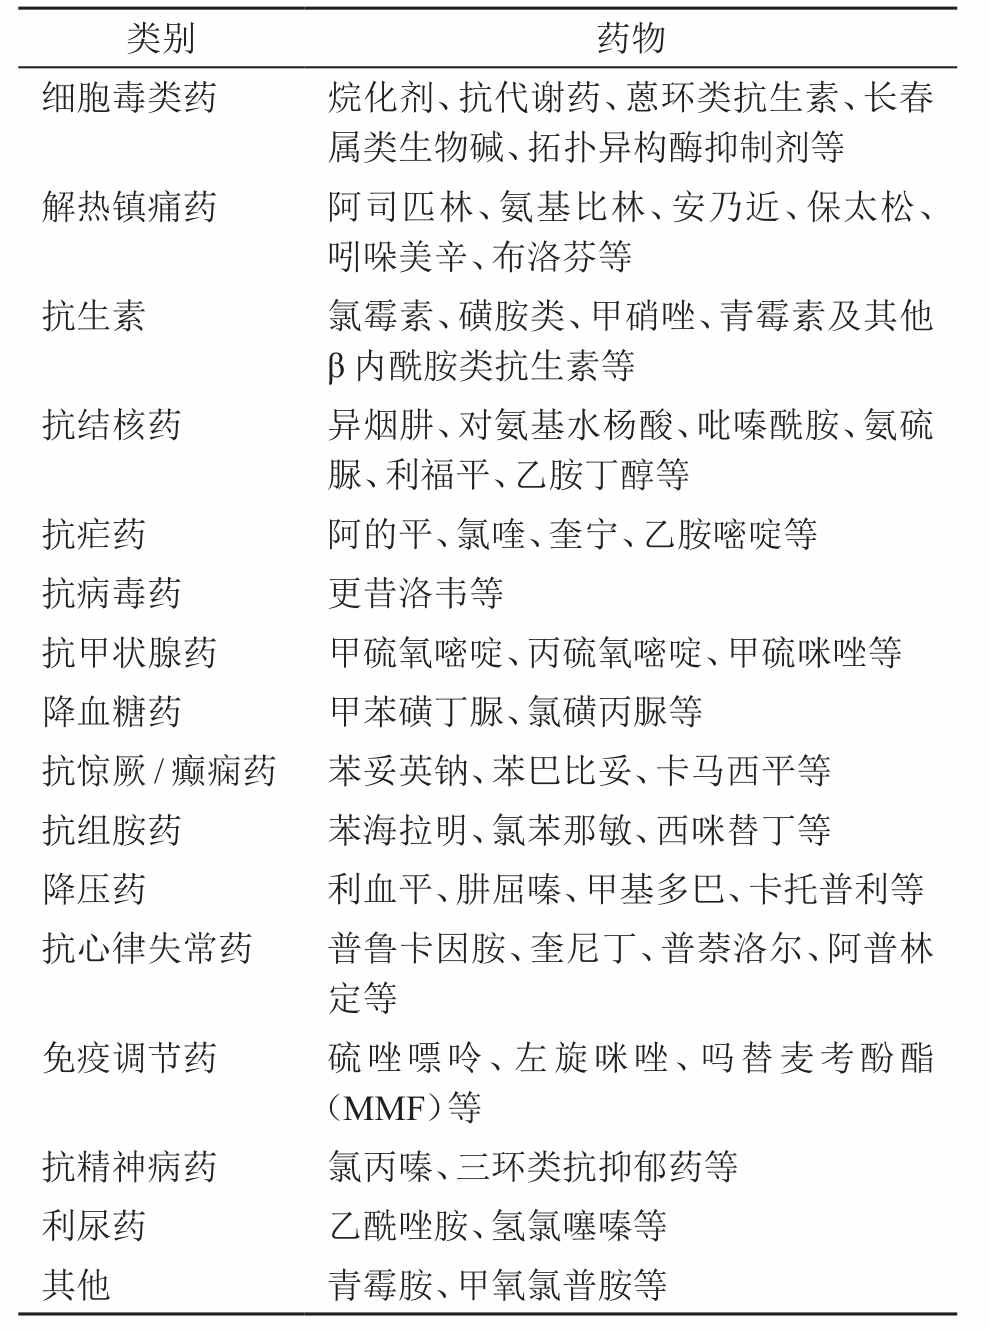
\includegraphics[width=3.29167in,height=4.42708in]{./images/Image00495.jpg}
\end{table}

\hypertarget{text00336.htmlux5cux23CHP12-2-1-1-1-4}{}
(4) 感染:

有些细菌、病毒、立克次体及原虫感染可引起粒细胞减少,多数是一过性的,其发病机制可能与中性粒细胞分布异常及破坏增多有关;有些如肝炎、艾滋病及细小病毒感染可引起中性粒细胞生成障碍;另有报道血行播散性结核通过T细胞介导使中性粒细胞生成受抑制。因此,其发病机制常是综合性的。

\hypertarget{text00336.htmlux5cux23CHP12-2-1-1-1-5}{}
(5) 骨髓浸润:

骨髓造血组织被白血病、骨髓瘤及转移癌细胞浸润,或大量成纤维细胞增生,影响正常造血干细胞增生,其结果不仅使中性粒细胞减少,也常伴贫血及血小板减少。

\hypertarget{text00336.htmlux5cux23CHP12-2-1-1-1-6}{}
(6) 某些先天性遗传性粒细胞减少症:

多数发病机制还不清楚,其中周期性中性粒细胞减少症被认为是一种常染色体显性遗传病,其机制是由于位于19p13.3上的中性粒细胞弹性蛋白酶基因(ELA2)突变所致。

\paragraph{成熟障碍}

维生素B\textsubscript{12}
或叶酸缺乏、急性粒细胞白血病、骨髓增生异常综合征以及某些先天性遗传性中性粒细胞减少等,骨髓分裂池细胞正常或增多,但由于粒细胞分化成熟障碍而在骨髓内死亡,导致贮存池成熟的中性粒细胞减少,因此也称无效增生。

\subsubsection{中性粒细胞在血液或组织中破坏或消耗过多}

\paragraph{免疫性因素}

中性粒细胞被抗体或抗原抗体复合物包裹在血液或脾等组织中被破坏,见于各种自身免疫性疾病(如系统性红斑狼疮、类风湿关节炎、Felty综合征)、某些非细胞毒类药物、某些感染(如慢性肝炎)及同种免疫性新生儿中性粒细胞减少。

\paragraph{非免疫性因素}

在严重细菌感染或败血症时,中性粒细胞在血液或炎症部位消耗增多;各种原因引起的脾大所致的脾功能亢进,中性粒细胞在脾内破坏增多。

\subsubsection{中性粒细胞分布异常}

中性粒细胞转移至边缘池导致循环池的粒细胞相对减少,但中性粒细胞总数并不减少,故多称为假性粒细胞减少,见于先天性或体质性假性粒细胞减少症。此外,获得性者如严重细菌感染、营养不良、疟疾等,常同时伴有中性粒细胞生成减少或破坏增多,故粒细胞总数也可减少。粒细胞滞留于循环池其他部位,如血液透析开始后2~15分钟滞留于肺血管内,导致外周血粒细胞暂时性减少;脾功能亢进时,滞留于脾内并常伴有破坏增多。

\subsection{诊断}

\subsubsection{病史}

1.注意询问细胞减少发生快慢 、频率、持续时间、减少程度和有无周期性
如果突然发生,最大可能是药物、放射线或感染所致。如呈周期性者,应考虑周期性中性粒细胞减少。如粒细胞长期减少,而红细胞及血小板始终正常,无药物或毒物接触史,无反复感染史、无相关疾病依据,则要进一步检查家族性或先天性中性粒细胞减少及假性粒细胞减少。

2.注意有无致病因素 特别是药物、毒物及放射线接触史。

3.注意有无相关疾病史
如急、慢性感染(包括肝炎、艾滋病)、类风湿关节炎、Felty综合征、系统性红斑狼疮及其他结缔组织病等。

4.家族史 注意家族成员有无相似患者。

\subsubsection{临床表现特点}

本病的临床表现,随其白细胞或中性粒细胞减少的原因、程度和时间长短而异。根据中性粒细胞减少的程度可分为轻度≥1.0
× 10\textsuperscript{9} /L、中度(0.5~1.0)× 10\textsuperscript{9}
/L和重度< 0.5 × 10\textsuperscript{9}
/L,重度减少者即为粒细胞缺乏症。一般轻度减少的患者临床上不出现特殊症状,多表现为原发病症状。中度和重度减少者易发生感染和出现疲乏、无力、头晕、食欲减退等非特异性症状。常见的感染部位是呼吸道、消化道及泌尿生殖道,可出现高热、黏膜的坏死性溃疡及严重的败血症、脓毒血症。粒细胞严重缺乏时,感染部位不能形成有效的炎症反应,常无脓液,X线检查无炎症浸润阴影或不明显;脓肿穿刺可无或有少量脓液。

\subsubsection{体检}

有无淋巴结、肝脾肿大、胸骨压痛及相关疾病的阳性体征和感染病灶。

\subsubsection{实验室检查}

\paragraph{血常规}

观察粒细胞减少的程度及是否伴有其他各系细胞减少和异常细胞。如为轻度减少,须重复检查,避免技术误差。对怀疑周期性中性粒细胞减少症者,应每周检查血常规2~3次,连续6周。

\paragraph{骨髓象}

对全血细胞减少者应同时进行骨髓涂片和活检,观察骨髓增生的程度、粒红比、分裂池和贮存池细胞百分率,有助于了解粒细胞减少的发病机制,为病因诊断提供线索。如果患者无贫血,红细胞系增生正常,当粒红比、分裂池和贮存池细胞百分率均减少时,表明粒细胞生成减少,可结合病史及其他检查去寻找病因。如果分裂池细胞百分率增高,粒红比及贮存池细胞百分率减低,表明是粒细胞成熟障碍或其生存期缩短。白血病、转移瘤等可见异常细胞浸润。中毒、药物和严重感染等所致的中性粒细胞缺乏症,可见粒细胞核固缩,胞浆内中毒性颗粒、空泡增多。再生障碍性贫血者骨髓增生受抑,三系减少。

\subsubsection{特殊检查}

\paragraph{肾上腺素试验}

肾上腺素可通过收缩小血管加快血流速度,使边缘池的中性粒细胞脱落进入循环池。此试验用以了解粒细胞是否分布异常。方法是皮下注射1∶1000肾上腺素0.2ml,注射后10、20及30分钟测定粒细胞数,如增多达原来的1倍或以上,且无脾大者,可诊断为假性粒细胞减少。

\paragraph{氢化可的松试验}

此试验是一种测定骨髓粒细胞贮备功能的方法,以鉴别中性粒细胞正常生理变动、慢性良性家族性粒细胞减少及药物等引起的粒细胞生成减少。方法是静脉滴注氢化可的松200mg后4~5小时,正常人粒细胞峰值较原来上升(4.5
± 0.5)× 10\textsuperscript{9} /L;慢性良性家族性粒细胞减少者上升(2.5 ±
0.4)× 10\textsuperscript{9} /L;药物等引起的粒细胞生成减少者上升(1.5 ±
0.3)× 10\textsuperscript{9}
/L或无反应。但要诊断慢性良性家族性粒细胞减少,尚需查家族成员。

\paragraph{中性粒细胞特异性抗体测定}

包括白细胞聚集反应、免疫荧光粒细胞抗体测定法等,以了解中性粒细胞的免疫状态。

\subsection{治疗}

\paragraph{病因治疗}

对可疑的药物或其他致病因素,应立即停止接触。继发性粒细胞减少者应积极治疗原发病。急性白血病、自身免疫性疾病、感染等经过治疗,病情缓解或控制后,中性粒细胞可恢复正常。脾功能亢进或Felty综合征所致的粒细胞减少脾切除治疗有效。

\paragraph{防治感染}

粒细胞缺乏患者的感染发生率极高,可达91.82\%,粒细胞计数越低,患者感染发生的风险就越高。粒细胞计数≤0.1
× 10\textsuperscript{9}
/L时,患者发生感染的比例最高。粒细胞缺乏患者极易发生院内感染,感染致病菌种类包括细菌、病毒、真菌、寄生虫等,与粒细胞缺乏持续时间相关。粒细胞缺乏患者的感染死亡率显著高于非粒细胞缺乏患者(46.48\%
vs
8.27\%)。当粒细胞缺乏患者出现发热症状时,应选择适当抗菌药物早期开始经验性治疗,2010年IDSA指南完善了粒细胞缺乏伴发热患者诊疗流程,增加了前期风险评估及治疗终点评估,调整了经验性用药方案推荐。

有预期较长(时间> 7天)及严重粒细胞减少(ANC≤0.1 ×
10\textsuperscript{9}
/L)和(或)伴有明显的并发症,如低血压、肺炎、新出现的腹痛或神经病学改变者为高危患者。这类患者需要入院接受经验性治疗,推荐单用抗假单胞菌β内酰胺类药物,如头孢吡肟,碳青霉烯类(美罗培南或亚胺培南-西司他丁),或哌拉西林-三唑巴坦治疗。也可在初始治疗方案基础上联合其他抗菌药物{[}氨基糖苷类、氟喹诺酮类和(或)万古霉素{]}用作有并发症(如低血压和肺炎),疑有或确诊为抗生素耐药时的治疗。不推荐万古霉素(或其他抗需氧革兰阳性球菌活性药物)作为发热和中性粒细胞减少时标准初始抗菌治疗方案的一部分。但有特定临床指征,包括疑为导管相关感染、皮肤和软组织感染、肺炎,或血流动力学不稳定时可考虑使用万古霉素。对于有下列抗生素耐药微生物感染危险的患者,尤其是患者病情不稳定或血培养结果阳性疑为耐药细菌感染时,可以修改初始经验性治疗。如耐甲氧西林金黄色葡萄球菌(MRSA),可考虑早期加用万古霉素、利奈唑胺或达托霉素;耐万古霉素肠球菌(VRE)考虑早期用利奈唑胺或达托霉素;产超广谱β内酰胺酶(ESBLs)革兰阴性杆菌考虑早期使用碳青霉烯类;产碳青霉烯酶(KPCs)考虑早期使用多黏菌素或替加环素等。

预期较短(时间≤7天)的粒细胞减少,无或少有并发症者为低危患者。这类患者应在门诊或住院处接受口服或静脉经验性抗菌治疗。口服经验性治疗推荐环丙沙星联合阿莫西林-克拉维酸,其他药物包括左氧氟沙星、克林霉素等。有持续发热(>
48小时)或感染恶化的症状体征时应再次住院或延长住院时间。

发热和中性粒细胞减少期间经验性抗菌治疗方案的更改应在临床和微生物资料指导下进行。经验性抗菌治疗的疗程取决于特定的微生物和感染的部位,适当的抗菌药物应持续用至中性粒细胞≥0.5
× 10\textsuperscript{9} /L,如临床需要,用药时间可再延长。

对于应用广谱抗生素4~7天仍持续性或反复发热的患者,以及中性粒细胞减少总时间预期>
7天者,应考虑经验性抗真菌治疗及进行侵袭性真菌感染的调查。对于已接受预防性抗真菌用药的患者,现有资料不足以推荐特别的经验性抗真菌药物,但可以考虑更换一种抗真菌药物静脉给药。对于高危中性粒细胞减少的亚组患者,可先发性应用抗真菌治疗来替代经验性抗真菌治疗。低危患者发生侵袭性真菌感染的风险较低,因此,不推荐常规应用经验性抗真菌治疗。抗念珠菌感染预防性给药推荐用于侵袭性念珠菌感染高危人群,如异体造血干细胞移植受者、因急性白血病接受密集缓解-诱导或解救-诱导化疗的患者。氟康唑、伊曲康唑、伏立康唑、泊沙康唑、米卡芬静或卡泊芬净都是可选用药。

\paragraph{升粒细胞药物}

造血生长因子,如重组人粒-单系集落刺激因子(rhGM-CSF)、重组人粒系集落刺激因子(rhG-CSF)治疗粒细胞缺乏症患者疗效明确,可使中性粒细胞迅速增多,并增强吞噬、杀菌及趋化功能。常用剂量为2~5μg/(kg•d),连续静脉滴注或分2次皮下注射。用药后中性粒细胞上升所需时间与增多数量和化疗等因素损伤干细胞的程度、骨髓造血恢复情况及个体差异等有关。常见的不良反应有发热、肌肉骨骼酸痛、皮疹等。一般用到粒细胞升至1.0
× 10\textsuperscript{9} /L左右即可停药。

\paragraph{免疫抑制剂}

自身免疫性粒细胞减少和通过免疫介导机制所致的粒细胞缺乏症,可用糖皮质激素等免疫抑制剂治疗。其他原因引起的中性粒细胞减少,则不宜采用。

\paragraph{粒细胞输注}

粒细胞半存期短、更新快,故粒细胞输注对慢性粒细胞减少治疗无意义。粒细胞输注的副作用很多,有时甚至很严重,故必须严格掌握适应证。目前主张只用于各种粒细胞缺乏合并严重感染,抗生素不能控制,且用rhGM-CSF或rhG-CSF未能提升至0.5
× 10\textsuperscript{9} /L时。

\paragraph{异基因骨髓移植}

只适用于重型再生障碍性贫血、获得性或先天性粒细胞缺乏合并严重免疫缺陷者。

\protect\hypertarget{text00337.html}{}{}

\hypertarget{text00337.htmlux5cux23CHP12-2-4}{}
参 考 文 献

1. 邓家栋
,杨崇礼,杨天楹,等.邓家栋临床血液学.上海:上海科学技术出版社,2001:911

2. Hoffman R,Benz Jr. EJ,Shattil SJ,et al. Hematology-Basic
Principles and Practice. 3th Ed. Beijing:Science press. 2001:743

3. Boxer L,Dale DC. Neutropenia:causes and consequences. Semin
Hematol,2002,39(2):75-81

4. Dale DC,Bolyard AA,Aprikyan A. Cyclic neutropenia. Semin Hematol.
2002;39(2):89-94

5. Berliner N,Horwitz M,Loughran TP Jr.,et al. Congenital and
Acquired Neutropenia. Hematology(Am Soc Hematol Educ
Program),2004,63-79

\protect\hypertarget{text00338.html}{}{}

